\documentclass[tikz,border=12pt]{standalone}
\usepackage{amsmath}
\usepackage{amssymb}
\usepackage{tikz}
\usetikzlibrary{arrows.meta}

\definecolor{ink}{HTML}{0F172A}
\definecolor{linegray}{HTML}{64748B}
\definecolor{visible}{HTML}{E2E8F0}
\definecolor{masked}{HTML}{F8FAFC}
\definecolor{maskedge}{HTML}{94A3B8}

\begin{document}
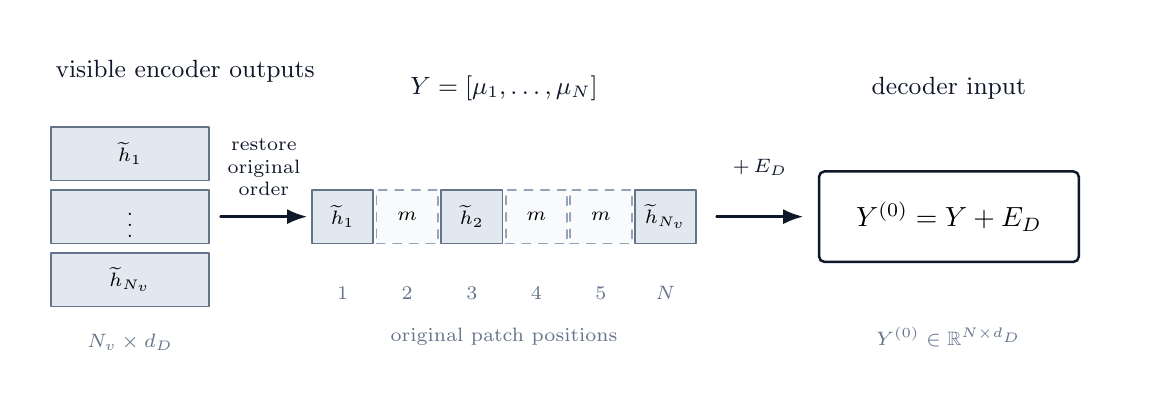
\begin{tikzpicture}[
  font=\sffamily,
  >=Latex,
  line cap=round,
  line join=round,
  token/.style={
    draw=linegray,
    line width=0.65pt,
    minimum width=0.78cm,
    minimum height=0.68cm,
    inner sep=1pt,
    fill=visible,
    font=\scriptsize
  },
  mask token/.style={
    token,
    draw=maskedge,
    dashed,
    fill=masked
  }
]
  \fill[white] (0,0) rectangle (14.2,4.55);

  % The encoder only returns the visible patch representations.
  \node[ink, font=\small] at (2.0,4.0) {visible encoder outputs};
  \node[token, minimum width=2.0cm] at (1.3,2.95) {$\widetilde{h}_1$};
  \node[token, minimum width=2.0cm] at (1.3,2.15) {$\vdots$};
  \node[token, minimum width=2.0cm] at (1.3,1.35) {$\widetilde{h}_{N_v}$};
  \node[linegray, font=\scriptsize] at (1.3,0.55)
    {$N_v\times d_D$};

  % Restore the original patch order and insert m at masked positions.
  \draw[ink, ->, line width=0.95pt] (2.45,2.15) -- (3.55,2.15);
  \node[ink, font=\scriptsize, fill=white, inner sep=1pt,
    text width=1.25cm, align=center] at (3.0,2.78)
    {restore\\original order};

  \node[ink, font=\small] at (6.05,3.78)
    {$Y=[\mu_1,\ldots,\mu_N]$};
  \node[token] at (4.0,2.15) {$\widetilde{h}_1$};
  \node[mask token] at (4.82,2.15) {$m$};
  \node[token] at (5.64,2.15) {$\widetilde{h}_2$};
  \node[mask token] at (6.46,2.15) {$m$};
  \node[mask token] at (7.28,2.15) {$m$};
  \node[token] at (8.1,2.15) {$\widetilde{h}_{N_v}$};

  \foreach \x/\position in {4.0/1,4.82/2,5.64/3,6.46/4,7.28/5,8.1/N} {
    \node[linegray, font=\scriptsize] at (\x,1.18) {$\position$};
  }
  \node[linegray, font=\scriptsize] at (6.05,0.62)
    {original patch positions};

  % Add positional information before the decoder.
  \draw[ink, ->, line width=0.95pt] (8.75,2.15) -- (9.85,2.15);
  \node[ink, font=\scriptsize, fill=white, inner sep=1pt] at (9.3,2.78)
    {$+\,E_D$};
  \node[ink, font=\small] at (11.7,3.78) {decoder input};
  \node[draw=ink, line width=0.9pt, rounded corners=2pt,
    minimum width=3.3cm, minimum height=1.15cm, fill=white,
    inner sep=4pt] at (11.7,2.15) {$Y^{(0)}=Y+E_D$};
  \node[linegray, font=\scriptsize] at (11.7,0.62)
    {$Y^{(0)}\in\mathbb{R}^{N\times d_D}$};
\end{tikzpicture}
\end{document}
